\chapter{La Matière Noire}

Dans le modèle de la cosmologie standard, la matière est composée à environ $80\%$ d'une matière invisible sans interaction avec le rayonnement électromagnétique~: on la désigne sous le nom de \textit{matière noire}. Cette matière est nécessaire pour expliquer notamment la distribution de matière aux plus grandes échelles, telle qu'elle est sondée par exemple par le fond diffus cosmologiques ou les grand relevés de galaxies. Elle est de fait un ingrédient essentiel du processus de formation des grandes structures de l'Univers, étudié plus en détail dans un chapitre dédié. Mais avant d'étudier cette formation, nous allons dédier un court chapitre aux indices en faveur de l'existence de cette matière et les quelques propriétés dont on pense qu'elle est pourvue. Cette matière n'est toutefois pas sans poser problème, en particulier aux échelles galactiques~: on décrira quelques-uns de ces problèmes ainsi que les pistes possible d'une réduction des tensions que pose cette matière noire.

\section{Matière noire et dynamique interne des structures}
L'une des indications les plus fameuses de l'existence de cette matière noire est la différence quasi-systématique entre la dynamique interne observée des grandes structures (galaxies, amas de galaxie) et celle prédite par son contenu lumineux.

\subsection{Courbe de rotation des galaxies}
L'exemple le plus connu est celui de la courbe de rotation plate des galaxies. La courbe de rotation désigne  la façon dont la vitesse de rotation de la matière dans un système auto-gravitant varie en fonction de la distance au centre de ce système. Par exemple, considérons une masse $M$ ponctuelle : un corps en orbite circulaire de rayon $r$ aura une vitesse de rotation donnée simplement par :
\begin{equation}
V_r(r)=\sqrt{\frac{GM}{r}}.
\end{equation} 
Ce comportement en $1/\sqrt{r}$ est par exemple celui observé dans le système solaire, où les corps les plus éloignés du Soleil sont aussi ceux qui orbitent le plus lentement. Pour un système étendu avec un profil de masse la relation reste inchangée:
\begin{equation}
V_r(r)=\sqrt{\frac{GM(<r)}{r}}.
\end{equation}
C'est la masse comprise à l'intérieur de l'orbite qui rentre en jeu : celle-ci peut augmenter avec le rayon\sidenote{par exemple un système de densité homogène voit $M(<r)\sim r^3$  et donc $V_r\sim r$ }, mais si il existe une distance au delà de laquelle cette masse ne varie plus \sidenote{comme attendu pour un système de taille finie}, on retrouve la décroissance standard en $1/\sqrt{r}$ de la vitesse de rotation.

On peut faire le même exercice dans une galaxie ou dans la Voie Lactée, en mesurant la vitesse de rotation des étoiles ou de la composante gazeuse du disque. Le résultat obtenu pour la Voie Lactée est présenté dans la figure \ref{f:rotcurve} : ce que l'on constate aisément c'est l'absence de décrochage de la vitesse de rotation dans la Galaxie et le maintien d'une vitesse constante, de l'ordre de 200 km/s, quelle que soit la distance considérée et ceci bien au delà de la limite du disque galactique (de l'ordre de 10 kpc). Ce type de courbe de rotation plate est représentatif de la cinématique d'un grand nombre de galaxies de type disque dans l'Univers et indique que la distribution de la matière ne s'arrête pas aux limite du disque galactique mais s'étend au delà \sidenote{c'est l'interprétation la plus standard, d'autres possibilités sont discutées en fin de chapitre}. Cette matière est invisible, plus étendue que la matière visible et permet le maintien de vitesse de rotation importantes de par son influence gravitationnelle : cette masse supplémentaire est nommée \textit{matière noire}.

\begin{figure}[htbp]
	\centering
		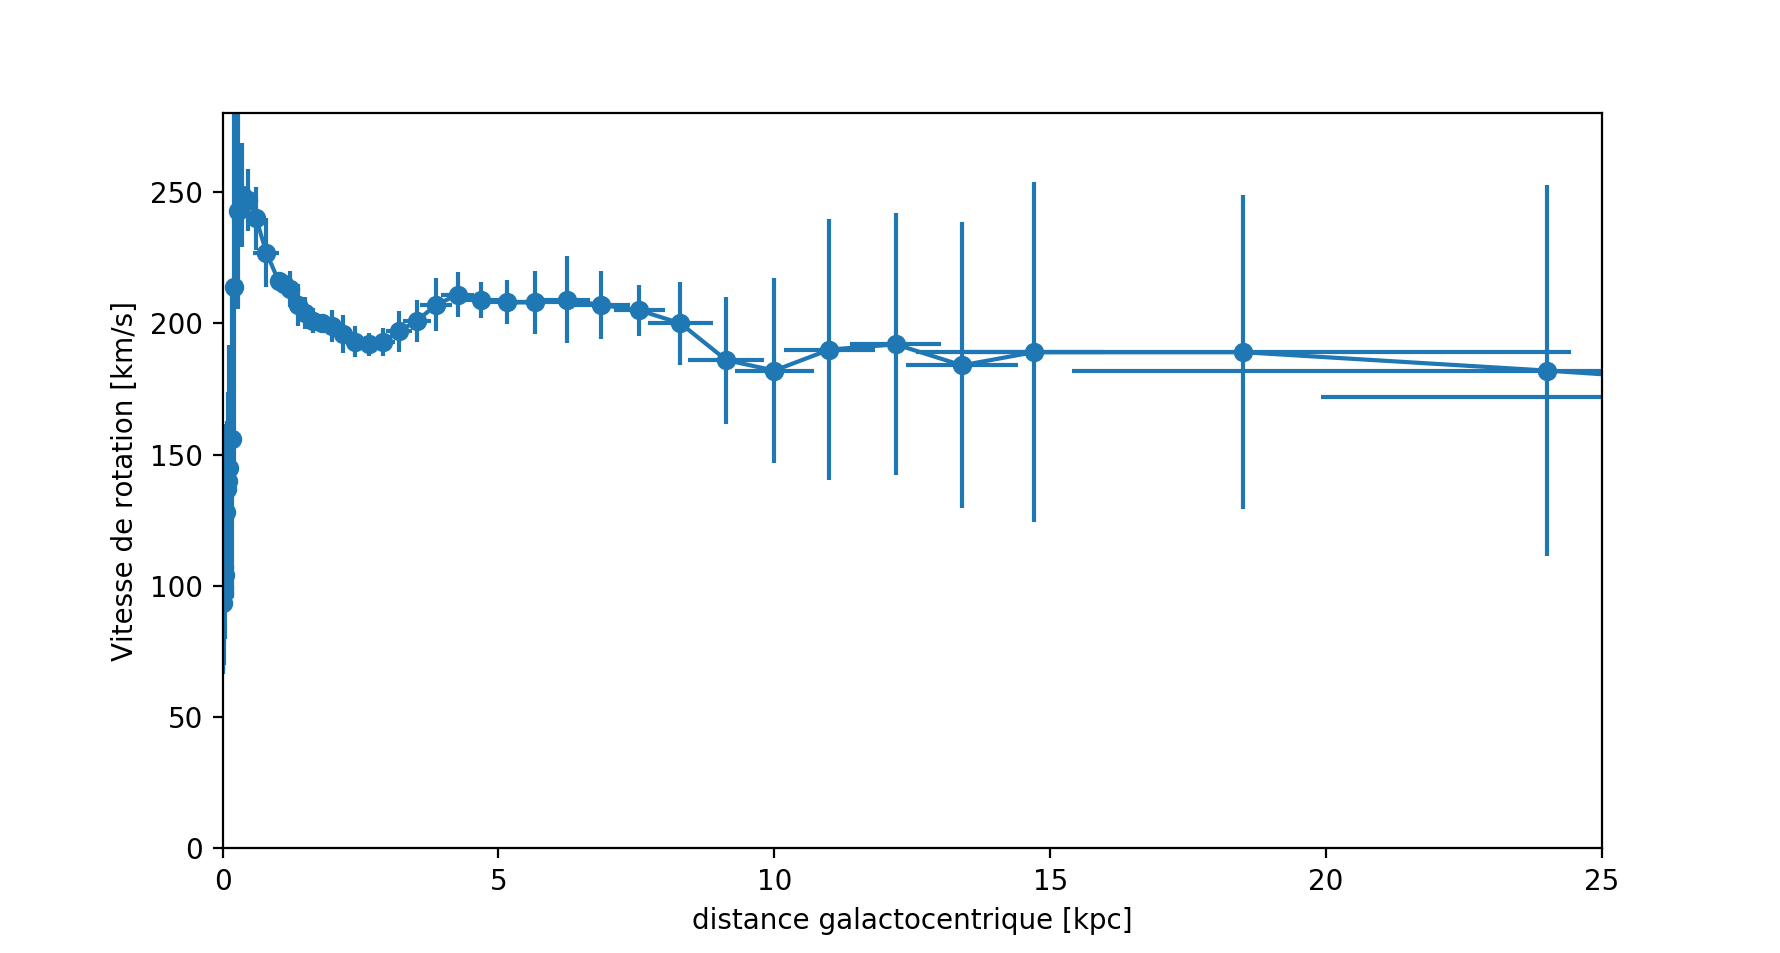
\includegraphics[height=20cm]{figs/rocurveMW.png}
	\caption{La vitesse de rotation de la matière dans la Voie Lactée en fonction de sa distance au centre, avec leurs incertitudes. Les points de données sont issus de Sofue (2013). Cette \textit{courbe de rotation} plate est représentative de la cinématique de la très grande majorité des galaxies de type disque dans l'Univers.} 
	\label{f:rotcurve}
\end{figure}

Un calcul rapide nous indique une masse dynamique pour la Voie Lactée que quelques $10^{11} M_\odot$, tandis que l'on estime la masse lumineuse (étoile + gaz) à environ 10 fois moins: non seulement la cinématique oblige à considérer une masse supplémentaire invisible mais sa contribution se doit d'être dominante.

\subsection{Amas de galaxie et théorème du Viriel}

Les galaxies de type disques ne sont pas les seules à présenter un désaccord entre la quantité de matière estimée par la production lumineuse et les sondes dynamiques. Historiquement\sidenote{dès 1933, par Zwicky} ce type de désaccord a d'abord été mis en évidence dans les amas de galaxies : ces structures dont la taille typique est de l'ordre du Mégaparsec\sidenote{donc environ 100 fois plus grandes que les galaxies} sont les plus grandes ayant pu se former au cours des 13 milliards d'années d'âge de l'Univers et peuvent contenir plusieurs centaines de galaxies.

Chacune de ces galaxies sont animées d'une vitesse propre permettant d'estimer la dispersion de vitesse $\sigma$ au sein de tels amas. Dans une situation d'équilibre, cette dispersion de vitesse est directement reliée à la masse totale du système. En effet, soit un système de N particules en interaction gravitationnelle, la particule $i$ obéit au principe fondamental de la dynamique:
\begin{equation}
m_i\frac{d^2 \vec{r_i}}{dt^2}=-\sum_{j\neq i}^N \frac{Gm_i m_j (\vec{r_i}-\vec{r_j})}{||\vec{r_i}-\vec{r_j}||^3}.
\end{equation}
Cette relation est satisfaite pour toutes les particules. Multiplions-la par $\vec{r_i}$ et additionnons toutes ces relations\sidenote{le passage de la 1ère à la 2ème ligne s'obtient en considérant la double somme comme la somme des deux parties triangulaires identiques au signe près d'une matrice NxN de diagnonale nulle} :
\begin{eqnarray}
\sum_i^N m_i\vec{r_i}\cdot\frac{d^2 \vec{r_i}}{dt^2}&=&-\sum_i^N \sum_{j\neq i}^N \frac{Gm_i m_j \vec{r_i}\cdot (\vec{r_i}-\vec{r_j})}{||\vec{r_i}-\vec{r_j}||^3}\\
&=& -\sum_i^N \sum_j^{i-1}\frac{Gm_i m_j}{||\vec{r_i}-\vec{r_j}||}\\
&=&E_{p,\mathrm{total}}.
\end{eqnarray}
On obtient l'énergie potentielle totale du système, définie comme étant la somme de toutes les énergies potentielles crées par les paires individuelles, sans redondance. Le terme de gauche peut se réecrire sous la forme:
\begin{eqnarray}
\sum_i^N m_i\vec{r_i}\cdot\frac{d^2 \vec{r_i}}{dt^2}&=&\frac{d^2}{dt^2}\sum_i^N m_i \vec{r_i}^2 - \sum_i^N m_i \left(\frac{d \vec{r_i}}{dt}\right)^2\\
&=&\frac{d^2}{dt^2}\sum_i^N m_i \vec{r_i}^2 - 2E_{c,\mathrm{tot}}.
\end{eqnarray}
On reconnaît l'énergie cinétique totale du système ainsi que la dérivée seconde du tenseur d'inertie au cours du temps\sidenote{plus précisément la dérivée de la trace du tenseur d'inertie}. Cette dernière quantité décrit la 'forme' du système : à l'équilibre la répartition des masses au sein du système doit rester constante et la dérivée du tenseur d'inertie doit être nulle. On obtient alors une expression du théorème du viriel:
\begin{equation}
2E_{c,\mathrm{tot}} + E_{p,\mathrm{total}} =0.
\end{equation}
En supposant l'équilibre, on peut estimer la masse totale d'un système si l'on est capable d'estimer son énergie cinétique. Par exemple pour l'amas de Coma, on mesure une dispersion des vitesses $\sigma \sim 1000$ km/s pour ses galaxies membres dans un rayon d'environ 3 Mégaparsec. Une application rapide du théorème de viriel permet d'écrire \sidenote{le facteur 3 dans l'énergie cinétique suppose une dispersion de vitesse isotrope dans les 3 directions tandis que l'énergie potentielle est celle d'un corps homogène } :
\begin{equation}
3M\sigma^2\sim \frac{3GM^2}{5R}
\end{equation}
conduisant à une estimation de sa masse de l'ordre de :
\begin{equation}
M\sim\frac{5R\sigma^2}{G}\sim 3\times 10^{15} M_\odot.
\end{equation}
Or on estime la masse lumineuse (dans les galaxies et sous la forme de gaz intra-amas) totale de l'amas de Coma à environ $1/10$ème de cette valeur. Ce désaccord entre masse dynamique et masse lumineuse est systématique dans les grands amas et illustre à nouveau le besoin d'une matière pesante non lumineuse en grande quantité.

\subsection{Halos de matière noire}

Les deux cours exemples précédents impose une image multi-phases des galaxies et des amas de galaxies: schématiquement une galaxie se compose d'une partie lumineuse composée d'étoiles, de gaz, de poussière et une partie sombre composée de matière noire. L'ajustement de modèles sur la dynamique observée des galaxies et des amas indique que cette matière est organisée en une composante plus étendue et moins dense que celle qui rayonne : les galaxies sont entourée d'un \textit{halo de matière noire}. Par exemple pour une galaxie comme la Voie Lactée, la masse de son halo est de l'ordre de $10^{11}-10^{12} M_\odot$ et son étendue est de l'ordre de quelques centaines de kiloparsecs. Rappelons qu'a proximité se trouve la galaxie d'Andromède légèrement plus massive et à une distance de 800 kiloparsecs environ : compte tenu de la faible séparation entre ces 2 objets, il est probable que les halos de ces 2 galaxies soient en contact.

Le rapport de masse entre la composante lumineuse et noire est d'environ $1/10$ème en défaveur de la matière lumineuse. Ce chiffre n'est pas si étonnant si l'on considère le rapport cosmique de la densité d'énergie de la masse baryonique et de la masse totale :
\begin{equation}
f_b=\Omega_b/\Omega_m\sim0.15.
\end{equation}
Ce rapport est appelé \textit{la fraction baryonique}: on retrouve le même ordre de grandeur que celui estimé précédemment. Pour l'essentiel, galaxies et amas ne font que conserver ce rapport universel. Ce n'est toutefois pas le cas des galaxies de très faible masse ($<10^{10} M_\odot$) : les modèles et les observations indiquent des fractions baryoniques plus faibles que la fraction universelle pour ces objets qui ne parviennent pas à piéger le gaz de façon aussi efficace que les structures plus massives. 
\begin{figure}[htbp]
	\centering
		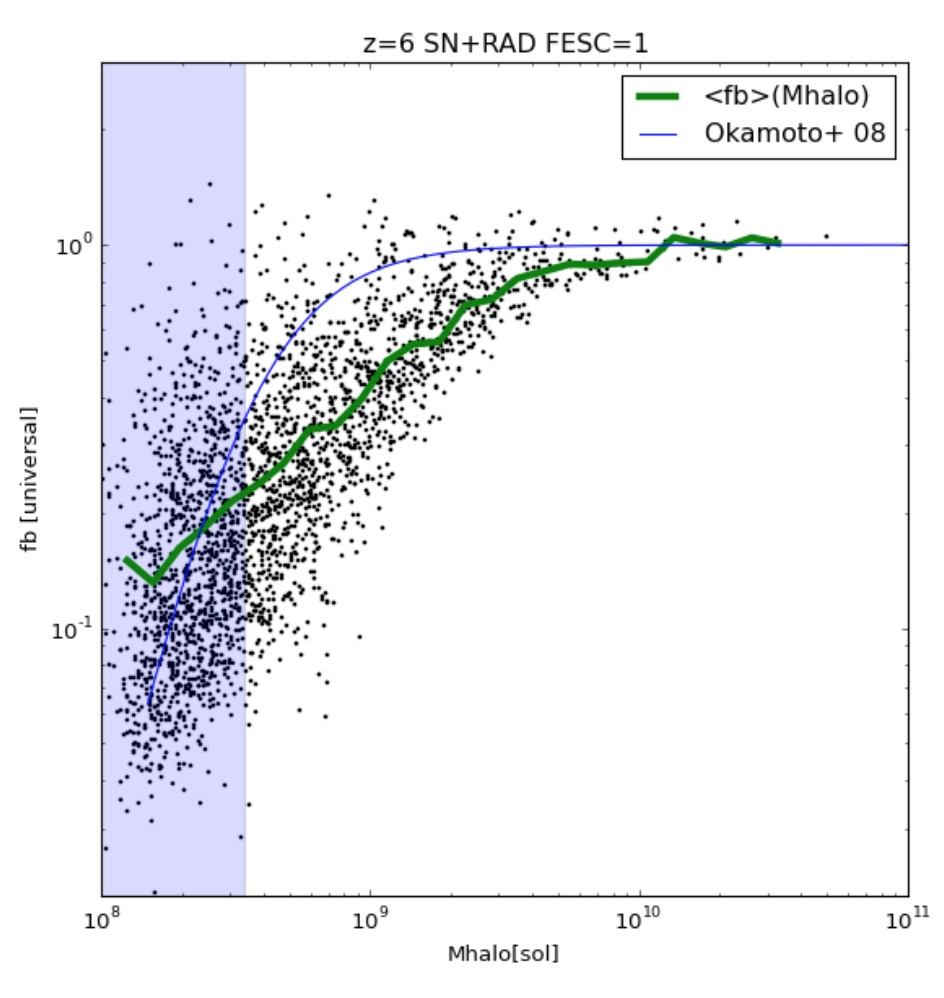
\includegraphics[height=8cm]{figs/fbar.png}
	\caption{La fraction baryonique prédite par une simulation numérique (points) et par un modèle de Okamoto+08 (ligne) environ 1 milliards d'années après le Big-Bang. On note le départ de cette fraction à la valeur universelle pour les objets de petite masse.} 
	\label{f:fbar}
\end{figure}

Ces petits objets sont particulièrement sensibles aux effets astrophysiques tels que l'éjection de gaz par l'explosion d'étoiles en supernovae ou le chauffage par le fond de rayonnement UV cosmique \sidenote{cf. le chapitre simulation}. Ils sont fortement dominés par la matière noire et sont donc des lieux idéaux pour l'étude de ses propriétés.
